\chapter{Subsystem: Environmental Sensing}


The environmental sensing subsystem includes the air quality sensors and video imaging array. The environmental sensing subsystem is an integral component of the fire monitoring functionality of the RSL Rover. It is the system that allows operators to gather visual and atmospheric information, an essential component for assessing fire-scene safety. The air quality sensors must display accurate information because they determine what gear is required to enter the area. The video imaging array is critical as it allows the operator to successfully see where the vehicle is within the environment, thus making it easy for the operator to drive through and visually inspect the environment. 

\section{Air Quality Assessment}

The air quality sensing subsystem consists of three redundant packages distributed on the front and top of the vehicle. Using three independent but redundant packages improve the accuracy of results since operators then have multiple values to compare against if there is a spike or other anomaly. It also allows a safety buffer if one or more sensors were to fail. Within each package there is an array of eight gas sensors, two temperature sensors with different temperature range sensitivities, an air particulate sensor, and a humidity sensor. The eight gas sensor array detects atmospheric concentration of the following: liquefied petroleum gas, carbon monoxide, carbon dioxide, natural gas, and hydrogen gas.

\subsection{Payload Requirements}

The list of important gases to detect was derived from the National Fire Protection Association handbook as they are the gases produced by a fire most hazardous to human life. Carbon dioxide is used as an indicator for fire because it is a primary product of complete combustion while carbon monoxide is a product of incomplete combustion. There are numerous components to smoke, most of which are hazardous, so the air particulate sensor is responsible for the detection of the smoke hazard indicator. In addition to the hazards produced from combustion, forest fires also increase the risk of residential gas leaks and explosions. Some jurisdictions use liquefied petroleum gas for residential heating and cooking while some use natural gas. Thus, liquefied petroleum gas and natural gas must both be detected to limit risks from gas fires. Atmospheric air temperatures can increase dramatically from large forest fires so it is important that the sensor package be able to detect fine changes at lower temperatures while still being able to detect high temperatures that are dangerous for firefighters. 

\subsection{Component Selection}
%Why we chose the various sensors and arduino

Gas sensors on the market are incredibly expensive, detect only a limited range of gases, and require complex, expensive calibration equipment. Instead of trying to implement this into the RSL Rover, we started from scratch and utilized the MQ-series sensors pictured in figure \ref{fig:MQSensor}.

\begin{figure}[h!]
	\centering
	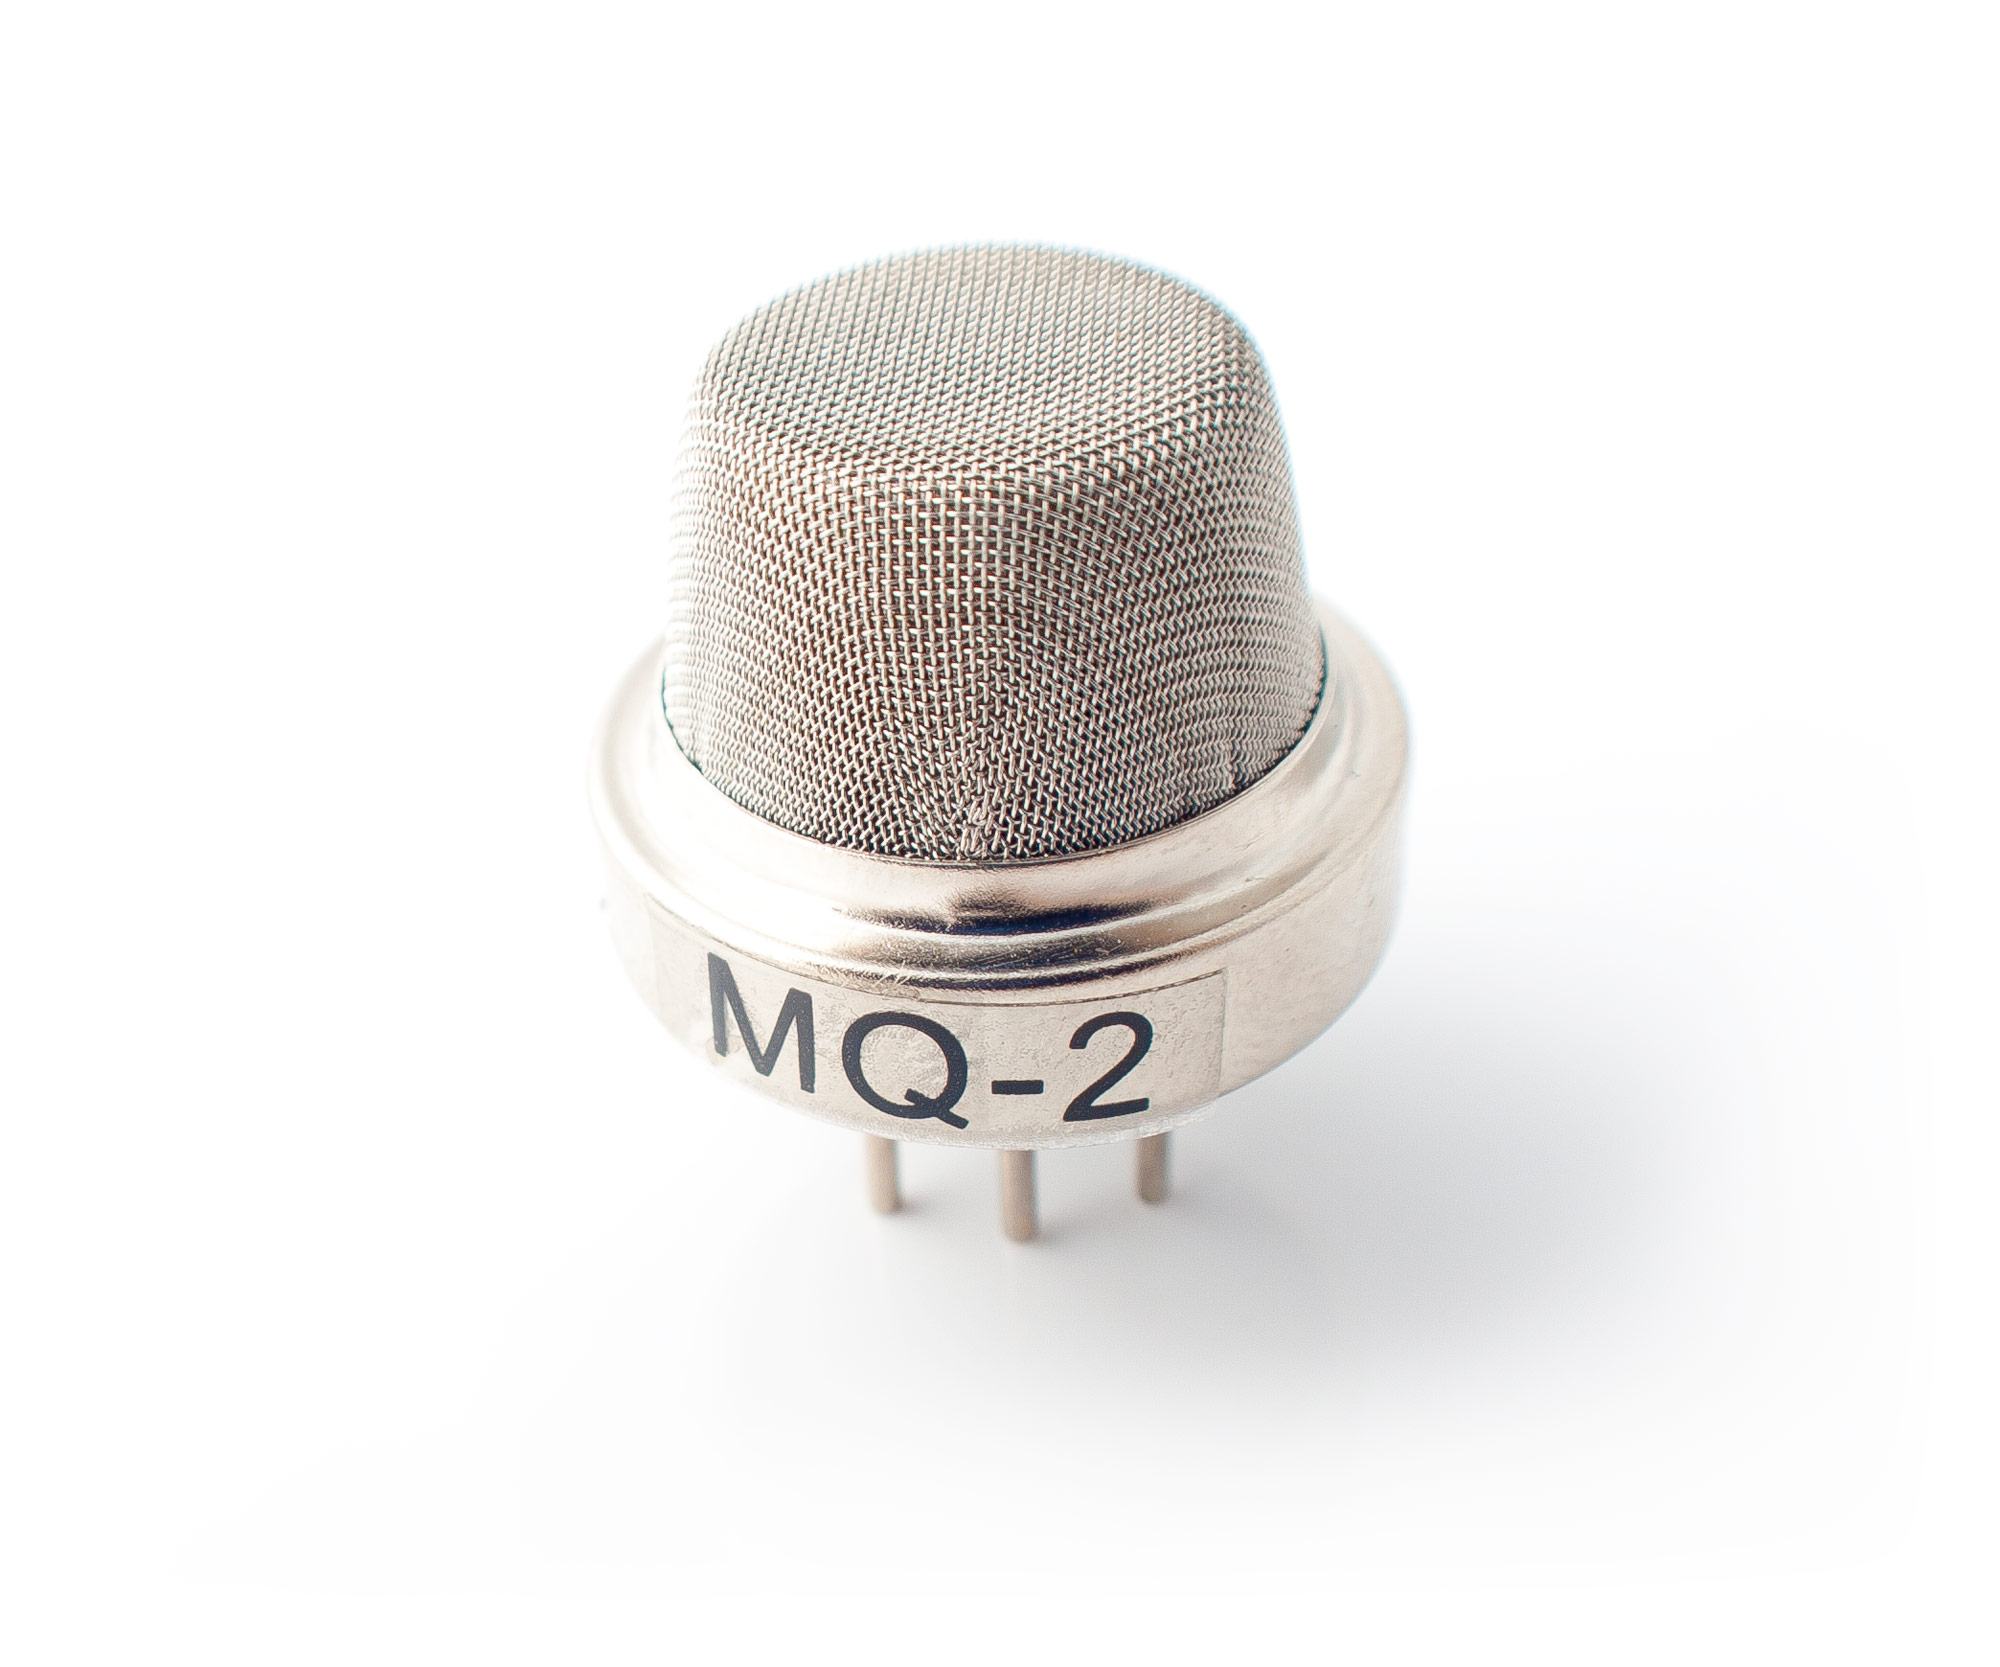
\includegraphics[scale=.1]{MQSensor.jpg}
	\caption{MQ-Series gas sensor}
	\label{fig:MQSensor}
\end{figure}

These sensors use a reactive filament that changes resistance according to the concentration of gases it is sensitive to. This makes for a robust, low cost solution that can easily be calibrated to show presence of a wide variety of gases. These sensors are sensitive to humidity, so a humidity sensor is also incorporated into the sensor package to allow for humidity corrections in the field. In addition, two temperature sensors are included to provide accurate temperature readings up to 250$^{\circ}$ Fahrenheit, which is beyond the safe limit for firefighters. The final sensing component was the air particulate sensor. For this, we utilized a Sharp GP2Y1010AU0F smoke and dust sensor picture in figure \ref{fig:SmokeDetector}. 

\begin{figure}[h!]
	\centering
	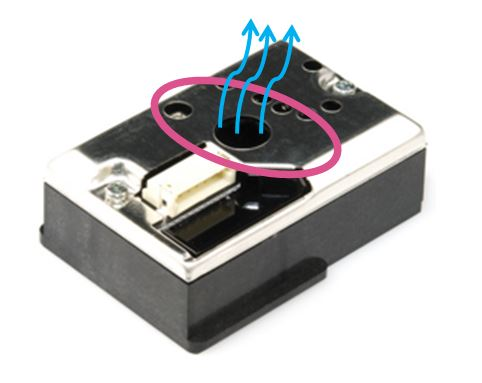
\includegraphics[scale=.6]{AirParticulateAirflow.jpg}
	\caption{Sharp air particulate sensor with air flow}
	\label{fig:SmokeDetector}
\end{figure}

The device works by pushing air through the center hole where it reflects infrared light off the smoke or dust. The more light that is reflected into the infrared receiver, the higher the smoke concentration is. The small voltage from the receiver is then amplified to a range of 0 to 3.3 Volts where 3.3 Volts is the maximum detectable concentration.

Each of these sensors requires its own circuitry and mounting hardware; to avoid large amounts of wiring and to give the sensors a place to sit, we created a printed circuit board that interfaces with each sensor. The board does not process the readings; an Arduino Mega 2560 is used to read and scale the analog voltages and digital readings from the sensor array. This is a low cost solution that allows for future modification as well as the planned modularity of the sensor package. The current printed circuit boards could be swapped out for a new circuit board with different sensing capabilities without having to change additional hardware. The data collected by the Arduino is processed on the onboard computer using ROS, limiting the impact on the Arduino.

\subsection{PCB Design}
%Mounted everything on custom PCB
%Problems that occurred after manufacturing
%include PCB layout and picture

We used kicad, a free CAD program, to design the entire circuit board. The first step was designing the schematic shown in figure \ref{fig:CircuitSchematic}.

\begin{figure}[H]
	\centerline{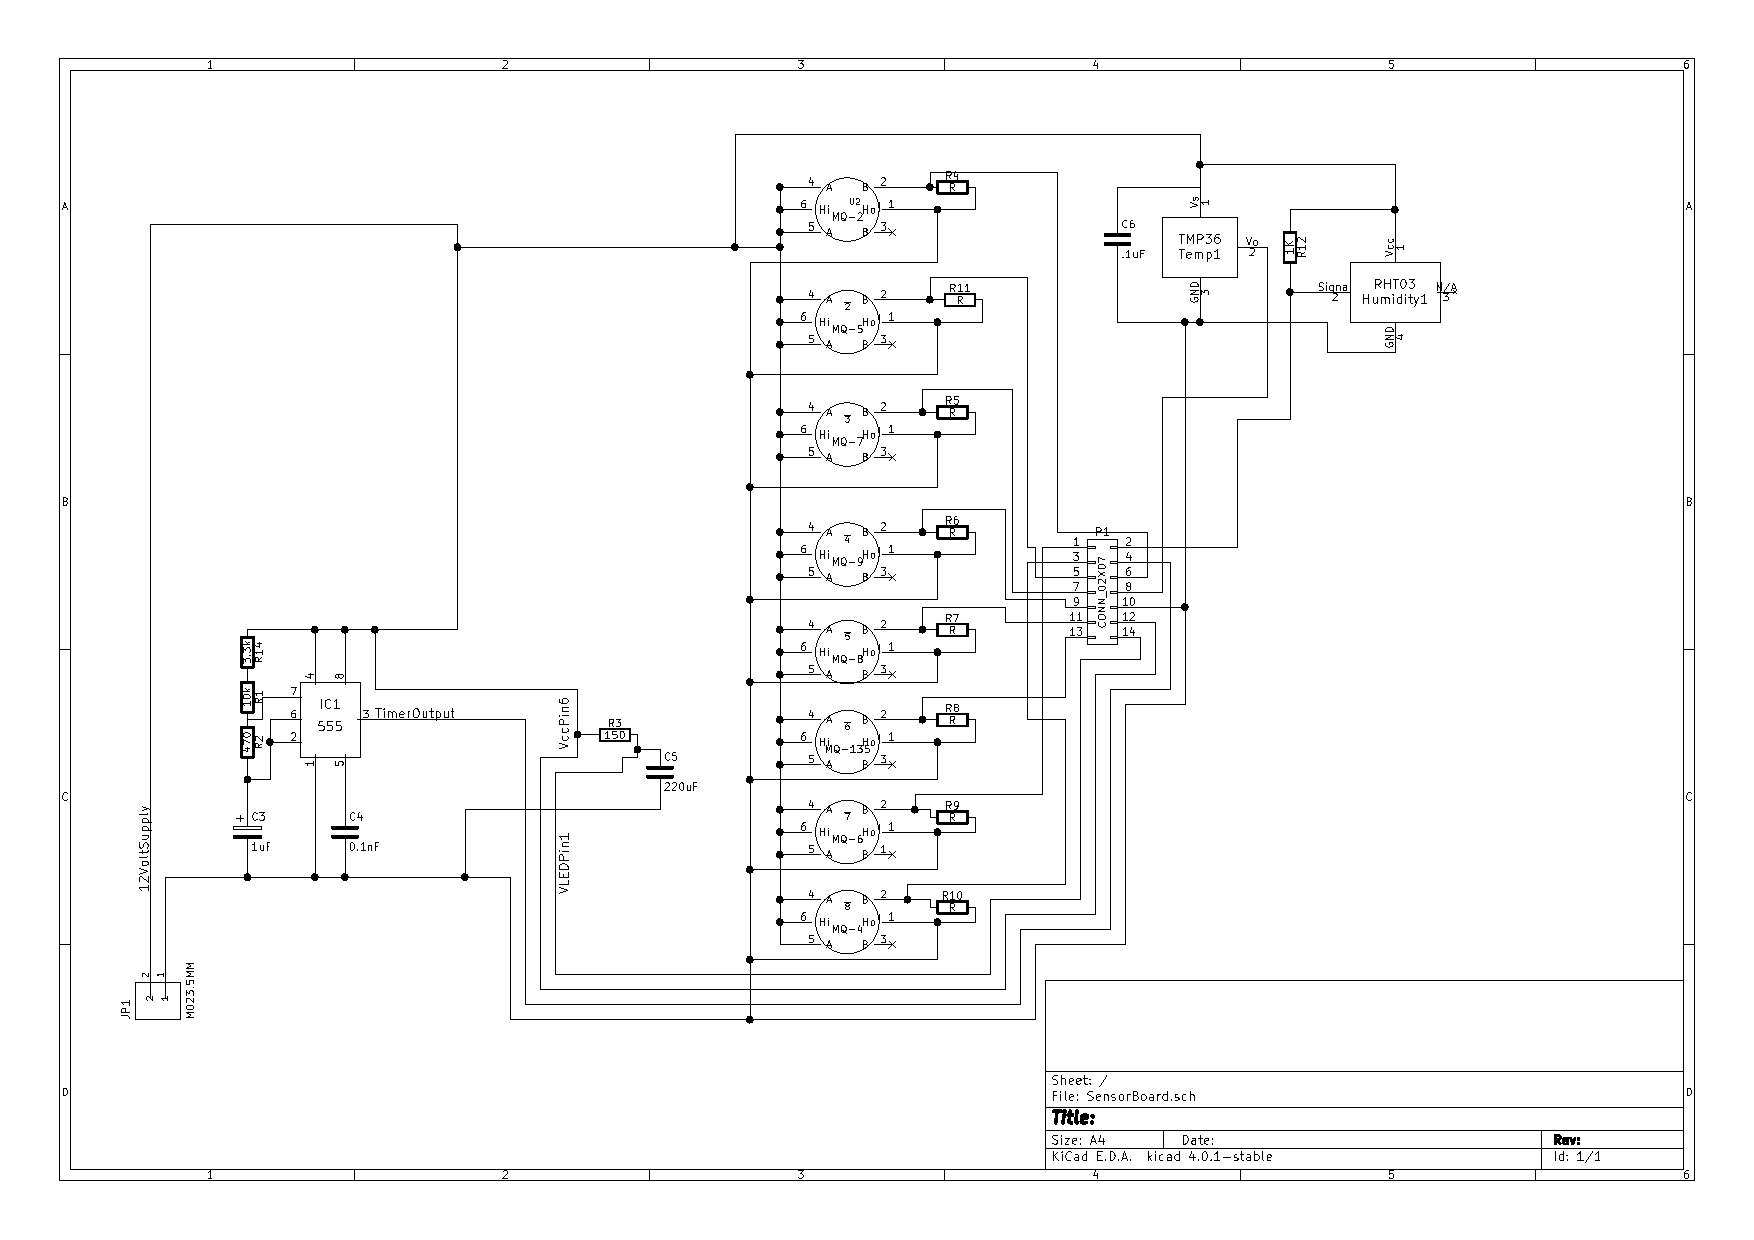
\includegraphics[width=1\linewidth]{images/SensorSchematic.pdf}}
	\caption{Air quality PCB schematic}
	\label{fig:CircuitSchematic}
\end{figure}

The schematic includes the timing circuit for the air particulate sensor, MQ sensor circuits, humidity hookups, and temperature circuits. Originally, a 12 Volt to 5 Volt regulating circuit was included in the schematic, but it was removed due to an overheating problem during testing. Instead, an external pulse width modulating regulator was added. The next step in designing the printed circuit board was laying out the circuits and component footprints in the layout editor. The final layout schematic is shown in figure \ref{fig:CircuitLayout}.

\begin{figure}[H]
	\centering
	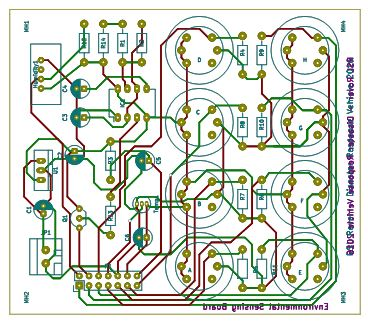
\includegraphics[scale=.8]{CircuitLayout.jpg}
	\caption{Printed circuit board layout}
	\label{fig:CircuitLayout}
\end{figure}

The design was sent to a board house where it was manufactured. We then populated the board with our sensors and tested. The first iteration had several problems, the most pronounced was the overheating of the voltage regulator. The regulator had to dissipate nearly 10 watts which caused it to get dangerously hot. We solved this by implementing a pulse width modulating voltage regulator and using a jumper wire across the original voltage regulator footprint. The next big problem we encountered was with the timer circuit for the air particulate sensor. The data sheet for the sensor showed an inverse graph of the required pulse form. To solve this, we simply removed the transistor that inverted the output from the 555 timer. All of these changes are shown in the schematic in figure \ref{fig:CircuitSchematic} but not the circuit board layout shown in figure \ref{fig:CircuitLayout}.

%\subsection{Manufacturing and Assembly}
%Include pictures of PCB in assembly

%\subsection{Calibration Procedure}

%\subsection{Data Processing}
%Potential subsection if turns out to be long
%Flowdown of arduino code
%Communication to ROS

\section{Cameras}

The camera system is a four camera array that provides a front facing view for the operator as well as a roughly 260\degree  view for observation of the surroundings. The initial design included four IP cameras, all of which ran as a unique node within the ROS network. ROS handles IP cameras over RTSP, the Real Time Streaming Protocol. This introduced an unacceptable amount of latency, about 4 seconds, to the camera stream. The final design includes four Logitech c615 usb cameras that are connected to a Raspberry Pi 2 Model B. A photo of the selected model of Logitech camera is included in Figure \ref{fig:logitechcam}. The dedicated Raspberry Pi runs an image of Ubuntu with ROS. The usb camera images are captured through ROS and sent through an OpenCV "person detection" application that recognizes bodies within the camera stream and outlines them in a green box so that they are visible to the operator. For an example of this capability, see Figure \ref{fig:peopledetect}. 

\begin{figure}[H]
	\centering
	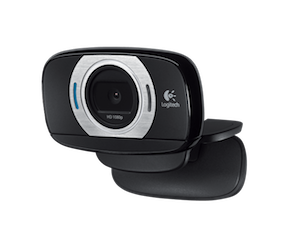
\includegraphics[scale=.7]{c615.png}
	\caption{Logitech c615 camera}
	\label{fig:logitechcam}
\end{figure}
\begin{figure}[H]
	\centering
	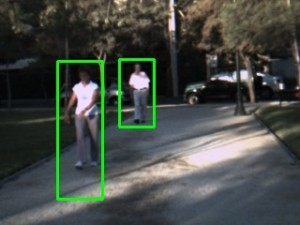
\includegraphics[scale=.7]{peopledetection.jpg}
	\caption{Example of OpenCV People Detection Application}
	\label{fig:peopledetect}
	\end{figure}

\section{Sensor and Camera Layout}

The location of the air quality sensors and cameras was a design decision. For the cameras, the field of view, mounting costs, implementation time and robustness, among other factors, were considered when deciding on a final design. Additionally, for the environmental sensors, the cost, implementation time, robustness and proximity to the vehicle's exhaust systems were considered when deciding on a sensor configuration. Appendix \ref{App:tradeoff} features a complete tradeoff analysis for the sensor configurations. A final configuration was chosen where the cameras are mounted on all 4 corners of the roll cage, allowing for a 360 degree view of the surroundings while also allowing the operator to see over obstacles. The redundant sensor packages are located on both sides of the front bumper and the center of the roll cage. 

%\section{Summary}